\section{Giải thuật di truyền (Genetic Algorithm)}

\subsection{Giới thiệu chung} % (fold)
\label{sub:Giới thiệu chung}

\begin{frame}{Giới thiệu chung}
Giải thuật di truyền là thuật toán có thể coi là cơ bản nhất trong tính toán
tiến hóa. Nó là một thuật toán tối ưu đơn mục tiêu, đơn nhiệm, nghĩa là nó chỉ
giải một bài toán tối ưu duy nhất:
\begin{align*}
  \min&\, f(x)\\
  \text{subject to}&\, x \in X
.\end{align*}

Mặc dù đơn giản, giải thuật di truyền có tính áp dụng rất cao. Chẳng hạn, nêu
cho $X$ là tập các mạng nơron (neural networks), hàm mục tiêu $f$ là hàm chi phí
(cost function) của các mạng nơron, thì thuật toán có thể được sử dụng để train
một mạng nơron mà không cần sử dụng khái niệm toán phức tạp như \textit{lan
truyền ngược} (backpropagation) với phương pháp giảm gradient.
\end{frame}

% subsection Giới thiệu chung (end)

\subsection{Thuật toán chung} % (fold)
\label{sub:Thuật toán chung}

\begin{frame}{Thuật toán chung}
Giải thuật di truyền sử dụng hai loại toán tử sinh sản:

\begin{itemize}
\item \textbf{Lai ghép} (crossover): tượng trưng cho sinh sản hữu tính. Lai ghép
  là quá trình sinh sản giữa hai cá thể cha mẹ và sinh ra một hoặc hai cá thể
  con. Khác với sinh sản hữu tính, lai ghép không phân biệt giới tính của cá thể
  cha mẹ, nghĩa là hai cá thể bất kỳ đều có thể tiến hành lai ghép với nhau.

\item \textbf{Đột biến} (mutation): tượng trưng cho sinh sản vô tính. Việc sinh
  ra thêm một cá thể giống y hệt cá thể cha mẹ của nó không chỉ không có ý
  nghĩa, mà còn làm mất đi độ đa dạng của quần thể, nên đột biến luôn làm thay
  đổi một cách ngẫu nhiên thông tin di truyền của cá thể cha mẹ để sinh ra cá
  thể con.

  Quá trình đột biến tạo ra sự đa dạng trong quần thể, đảm bảo \textbf{tính đa
  dạng} trong ba điều kiện của chọn lọc tự nhiên.
\end{itemize}
\end{frame}

\begin{frame}[fragile]
\frametitle{Thuật toán chung}
  Sử dụng hai toán tử này, cùng với toán tử chọn lọc, ta thu được thuật toán
  chung của giải thuật di truyền như sau:
\begin{minted}[fontsize=\scriptsize]{python}
def ga():
  population = init_pop() # khởi tạo quần thể
  while True:
    new_population = [] # mảng lưu các quần thể mới

    for _ in range(POP_SIZE / 2):
      # chọn ra các cá thể cha mẹ để thực hiện lai ghép
      p1, p2 = select_parents(population)
      # thực hiện lai ghép `p1` và `p2` sinh ra `c1` và `c2`
      c1, c2 = crossover(p1, p2)
      # với xác suất `mutation_rate`, thực hiện đột biến
      if random.random() < mutation_rate: mutate(c1)
      if random.random() < mutation_rate: mutate(c2)

      new_population += [c1, c2] # thêm `c1` và `c2` vào quần thể mới
    population = new_population
    yield population
\end{minted}
\end{frame}

% subsection Thuật toán chung (end)

\subsection{Khởi tạo quần thể} % (fold)
\label{sub:Khởi tạo quần thể}

\begin{frame}[fragile]
\frametitle{Khởi tạo quần thể}
Theo lý thuyết, do giải thuật tiến hóa đã có được ba điều kiện của chọn lọc tự
nhiên (tính đa dạng nhờ toán tử đột biến), nên hầu hết mọi quần thể ban đầu đều
sẽ tiến hóa và hội tụ đến một nghiệm tương đối tối ưu.

Tuy nhiên, ta nên lưu ý khởi tạo quần thể ban đầu cho đa dạng nhất có thể, nghĩa
là phương pháp tự nhiên nhất là cho các cá thể ban đầu có cùng một kiểu gen mặc
định nào đó không phải là một ý tưởng tốt.

Vì thế, ta sử dụng cách tự nhiên thứ hai: \textbf{khởi tạo quần thể một cách
ngẫu nhiên}:
\begin{minted}{python}
# hàm khởi tạo quần thể
def init_pop():
  # tạo ra một list gồm `POP_SIZE` phần tử (tham số cho trước)
  # mỗi phần tử là một kết quả từ hàm `random_individual`,
  # một cá thể ngẫu nhiên
  return [random_individual() for _ in range(POP_SIZE)]

\end{minted}
\end{frame}

\begin{frame}[fragile]
\frametitle{Khởi tạo quần thể}
Việc tạo ra một cá thể ngẫu nhiên sẽ được cài đặt tùy vào cách mã hóa cá thể.
Chẳng hạn, với một vector trong \( [0, 1]^{D} \), thì ta có thể lấy mỗi phần tử
của vector ngẫu nhiên từ 0 đến 1 một cách độc lập.

Tuy nhiên, với chẳng hạn là mã hóa của một đường đi Hamilton của đồ thị, bắt
buộc phải có dạng là một hoán vị của tập số chỉ của các đỉnh, ta cần phải đảm
bảo tính chất này mà không lấy ngẫu nhiên một cách bừa bãi.

\begin{minted}{python}
from itertools import permutation # khai bào thư viện
# tập số chỉ của đỉnh, gồm các số nguyên từ 1 đến 10
V = range(1, 10)

def random_individual_hamiltonian_path(): return permutation(V)
# kết quả có thể: [1, 3, 6, 2, 9, 7, 8, 4, 10, 5]
\end{minted}
\end{frame}
% subsection Khởi tạo quần thể (end)

\subsection{Toán tử chọn lọc} % (fold)
\label{sub:Toán tử chọn lọc}

\begin{frame}[fragile]
  \frametitle{Toán tử chọn lọc}
  Trong giải thuật di truyền, toán tử chọn lọc được sử dụng để chọn ra các cá
  thể cha mẹ để lai ghép, chứ không được sử dụng nhằm loại bỏ đi các cá thể
  không tốt khỏi quần thể.

  Nếu ở đây, ta chọn các cá thể cha mẹ một cách hoàn toàn ngẫu nhiên, thì quá
  trình chọn lọc sẽ không phân biệt được giữa cá thể kém và cá thể tốt, làm cho
  giải thuật không bao giờ tốt hơn được.

  Còn nếu ta chỉ chọn các cá thể cha mẹ là hai cá thể tốt nhất, thì thế hệ sau
  sẽ chỉ gồm các cá thể giống các cá thể này, làm giảm đi độ đa dạng quần thể
  một cách đáng kể.

  Do vậy, quá trình chọn lọc cần phải cân bằng giữa việc chọn các cá thể tốt và
  cá thể không tốt.
\end{frame}

\begin{frame}[fragile]
  \frametitle{Toán tử chọn lọc}

  Một phương hướng tự nhiên để cài đặt toán tử chọn lọc là lấy giá trị hàm
  fitness làm trọng số để chọn ngẫu nhiên:

  \begin{minted}{python}
import random

def select_parents(population):
  # mảng gồm các giá trị fitness của từng cá thể
  weights = [fitness(individual) for individual in population]
  return random.choices(population,
                        weights, # trọng số lấy ngẫu nhiên, tỉ
                                 # lệ với xác suất được lấy ra.
                        k=2)     # `k` là số phần tử được chọn
  \end{minted}

  Cách này có tên gọi là \textbf{Roulette Wheel Selection} (chọn lọc bánh xe).
\end{frame}

\begin{frame}{Toán tử chọn lọc}
  Roulette Wheel Selection, nếu như hàm fitness là một hàm chênh lệch lớn, sẽ có
  thể làm cho trọng số của một số các cá thể tốt rất lớn so với các cá thể còn
  lại. Do đó, các cá thể còn lại có thể hầu như không được chọn, nghĩa là quần
  thể sẽ mất đa dạng đi một lượng đáng kể.

  Để khắc phục vấn đề này, thay vì dùng trực tiếp giá trị hàm fitness làm
  trọng số, ta có thể tính toán các trọng số thông qua \textbf{thứ tự của các cá
  thể khi sắp xếp theo giá trị hàm fitness}. Cách làm này được gọi là
  \textbf{Rank Selection}.

  Một cách tổng quát, ta sẽ tính trọng số của cá thể thứ $i$ (sau khi sắp xếp
  theo thứ tự từ tốt đến kém)
  bẳng một hàm $w(i)$, thỏa mãn $w(i) \ge w(j), \forall 1 \le i \le j \le n$ (\(
  n\) là số cá thể của quần thể trước bước chọn lọc).

  Từ hàm trọng số, ta có thể tính trực tiếp luôn xác suất:
  \[
    P(i) = \frac{w(i)}{\sum_{k = 1}^{n} w(k)} = \frac{w(i)}{W_{n}}
  .\] 
\end{frame}

\begin{frame}{Toán tử chọn lọc}
  Một hàm $w$ hay được sử dụng cho Rank Selection là chọn lọc tuyến
  tính của Baker. Hàm $w$ thực chất là nội suy tuyến tính giữa một hàm
  hằng số (\( w_{c}(i) = 1 \)) và hàm thuần hạng (\( w_{r}(i) = 2\frac{n - i}{n - 1}
  \)), với tham số nội suy \( t \in [0, 1] \).
  
  Hệ số $2$ trong biểu thức của $w_{r}$ có mục đích làm cho tổng trọng số của
  hai hàm bằng nhau:
  \begin{align*}
    \sum_{i = 1}^{n} w_{r}(i) &= 2 \cdot \frac{0 + 1 + 2 +\ldots + (n - 1)}{n
    -1} = n\\
    \sum_{i = 1}^{n} w_{c}(i) &=  n
  .\end{align*}
\end{frame}

\begin{frame}
\frametitle{Toán tử chọn lọc}
  Do đó, tổng trọng số của hàm $w$ không phụ thuộc vào tham số $t$, và bằng $n$:
  \begin{align*}
    W_{n} &= \sum_{i = 1}^{n} w(i)\\
    &= \sum_{i = 1}^{n} \left( w_{c}(i) + t(w_{r}(i) - w_{c}(i)) \right)  \\
    &= n + t (n - n) = n.
  \end{align*}

  Đặc điểm này làm công thức xác suất đơn giản hơn và thực sự là một hàm bậc
  nhất theo biến $t$.
\end{frame}

\begin{frame}{Toán tử chọn lọc}
  Sau khi tính được $W_{n}$, ta quay lại tính hàm trọng số $w(i)$ và hàm xác
  suất $P(i)$:
  \begin{align*}
    w(i) &= w_{c}(i) + t(w_{r}(i) - w_{c}(i))\\
    &= 1 + t \left( 1 - 2\frac{n - i}{n - 1} \right)
  .\end{align*}
  Nếu ta cho \( sp = 1 + t \in [1, 2]  \), ta viết lại \( w(i) \) dưới dạng
  chính gốc là:
  \begin{align*}
    w(i)
    &= 1 + t \left( 1 - 2\frac{n - i}{n - 1} \right)\\
    &= (1 + t) - 2t \left( 1 - \frac{n - i}{n - 1} \right)  \\
    &= sp - (2sp - 2) \frac{i - 1}{n - 1}\\
    \implies P(i) &= \frac{1}{n} \left( sp - (2sp - 2) \frac{i - 1}{n - 1} \right) 
  \end{align*}
\end{frame}

\begin{frame}[fragile]
\frametitle{Toán tử chọn lọc}
  Ngoài các toán tử chọn lọc sử dụng trọng số, ta cũng có một cách chọn lọc đơn
  giản hơn mà chỉ sử dụng chọn lọc ngẫu nhiên đều. Thay vì ta lấy các cá thể tốt
  nhất của cả quần thể và làm mất đi tính đa dạng như cách chọn lọc ngây thơ đã
  nói trên, ta có thể lấy ra một nhóm nhỏ từ quần thể gồm có \( k \) cá thể, sau đó
  chọn lọc ra cá thể tốt nhất trong nhóm này. Cách này được gọi là
  \textbf{Tournament Selection}.

  Theo cách này, mọi cá thể trong top \( n - k + 1 \) các cá thể tốt nhât đều có
  thể được chọn, và cá thể càng tốt sẽ càng có xác suất được chọn lớn hơn (vì nó
  là cá thể tốt nhất trong nhiều nhóm hơn).
  \begin{minted}[fontsize=\scriptsize]{python}
import random

def select_parents(population):
  # lấy hai nhóm cho hai cá thể cha mẹ
  group_1 = random.sample(population, k)
  group_2 = random.sample(population, k)

  # trả lại hai cá thể tốt nhất của hai nhóm
  return max(group_1, key=fitness), max(group_2, key=fitness)
  \end{minted}
\end{frame}

\begin{frame}[fragile]
\frametitle{Toán tử chọn lọc}
Các toán tử chọn lọc trên có thể được sử dụng để chọn cha mẹ hoặc chọn các cá
thể để giữ lại. Ngoài ra, ta còn có một số toán tử chọn lọc chỉ có thể áp dụng
để giữ lại các cá thể:

\begin{itemize}
\item \textbf{Truncation Selection}: chọn lọc lấy top $N$ của quần thể theo
  hàm fitness, như đã trình bày ở phần mở đầu.

\item \textbf{Stochastic Selection}: ta sử dụng trọng số (tính như Roulette
  Wheel Selection hoặc Rank Selection) để làm độ dài cho một đoạn tượng trưng
  cho mỗi cá thể, nối tiếp các đoạn này để phủ kín \( [0, W_{n}] \), sau đó chọn
  các cá thể có đoạn chứa các điểm \( r, r + \frac{W_{n}}{n}, r + 2
  \frac{W_{n}}{n}, \ldots , r + (n - 1) \frac{W_{n}}{n} \), với $r$ là một số
  ngẫu nhiên được chọn từ $\left[ 0, \frac{W_{n}}{N} \right]$.

\begin{figure}
  \centering
  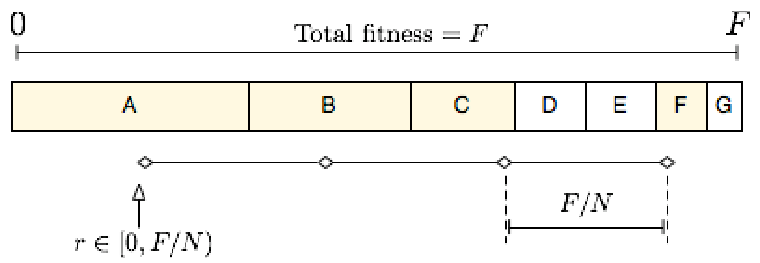
\includegraphics[width=.8\textwidth,height=0.25\textheight,keepaspectratio]
  {res/stochastic.png}
\end{figure}
\end{itemize}
\end{frame}

\begin{frame}[fragile]
\frametitle{Toán tử chọn lọc}
Để đảm bảo thế hệ sau ít nhất là tốt bằng thế hệ trước (tính theo cá thể tốt nhất của
mối thể hệ), người ta có thể đưa thêm một nhóm nhỏ các cá thể tốt nhất từ thế hệ
trước sang thế hệ sau đó. Đây được gọi là \textbf{Elitist Selection}, và nó có
thể được kết hợp với các toán tử chọn lọc trên.

Khi sử dụng \textbf{Elitist Selection}, do thế hệ sau sẽ luôn ít nhất tốt bằng
thế hệ trước, nên nếu hàm mục tiêu bị chặn, thì dãy $f_{i}$ - fitness của cá thể
tốt nhất trong thế hệ thứ $i$ là một dãy không giảm và bị chặn, do đó luôn hội
tụ đến một giá trị nào đó.

Do vậy, giải thuật di truyền luôn hội tụ đến một nghiệm tối ưu địa phương, về
mặt lý thuyết. Tuy nhiên nó có thể mất rất nhiều thế hệ để có thể thực sự tiến
gần đến điểm này.
\end{frame}

% subsection Toán tử chọn lọc (end)

\subsection{Toán tử lai ghép} % (fold)
\label{sub:Toán tử lai ghép}

\begin{frame}{One-point crossover và N-point crossover}
  \textbf{One-point crossover} (lai ghép một điểm) là một toán tử lai ghép nảy
  sinh tự nhiên như cái tên "crossover" của lai ghép.

  Khi hai nhiễm sắc thể trong thực tế thực hiện lai ghép, chúng trao đổi chéo
  với nhau (crossing over), một đoạn của nhiễm sắc thể này được chuyển sang
  nhiễm sắc thể kia và ngược lại.

\begin{figure}[t!]
    \centering
    \begin{subfigure}[t]{0.5\textwidth}
        \centering
        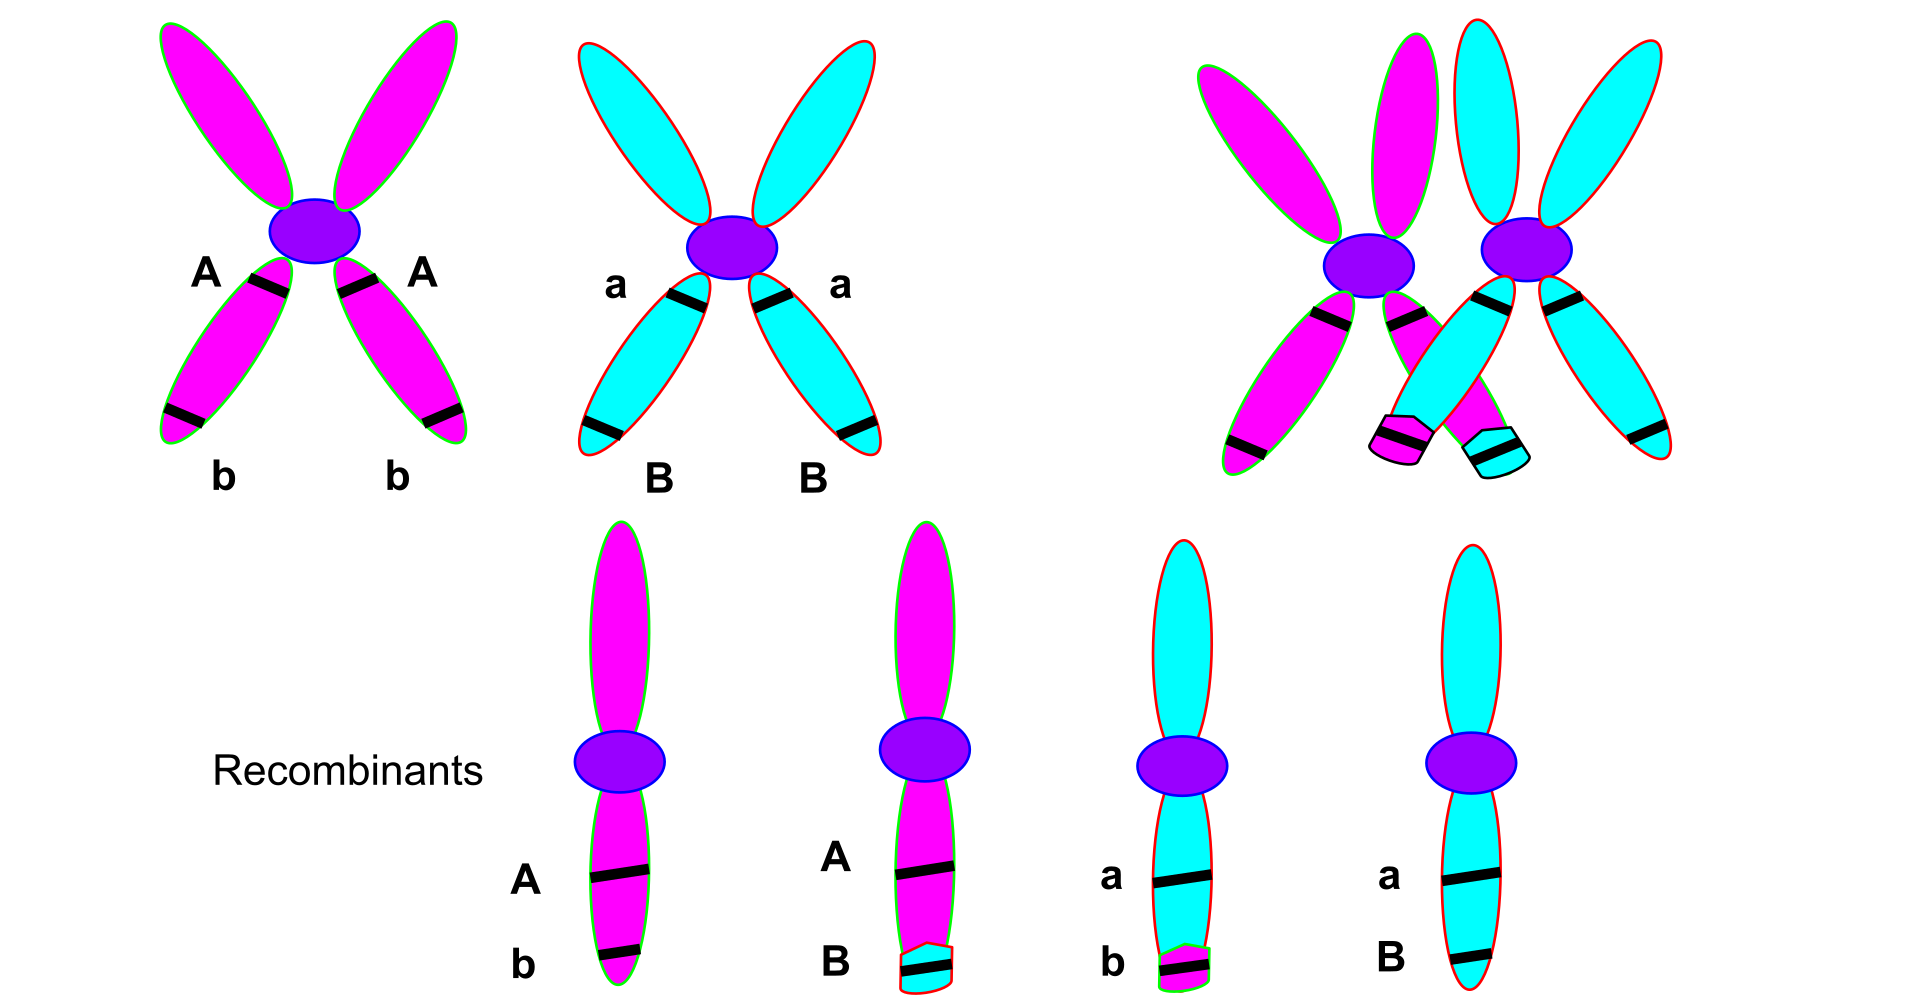
\includegraphics[height=1.2in]{res/chromosomal.png}
        \caption{Trao đổi chéo giữa hai nhiễm sắc thể}
    \end{subfigure}%
    ~ 
    \begin{subfigure}[t]{0.5\textwidth}
        \centering
        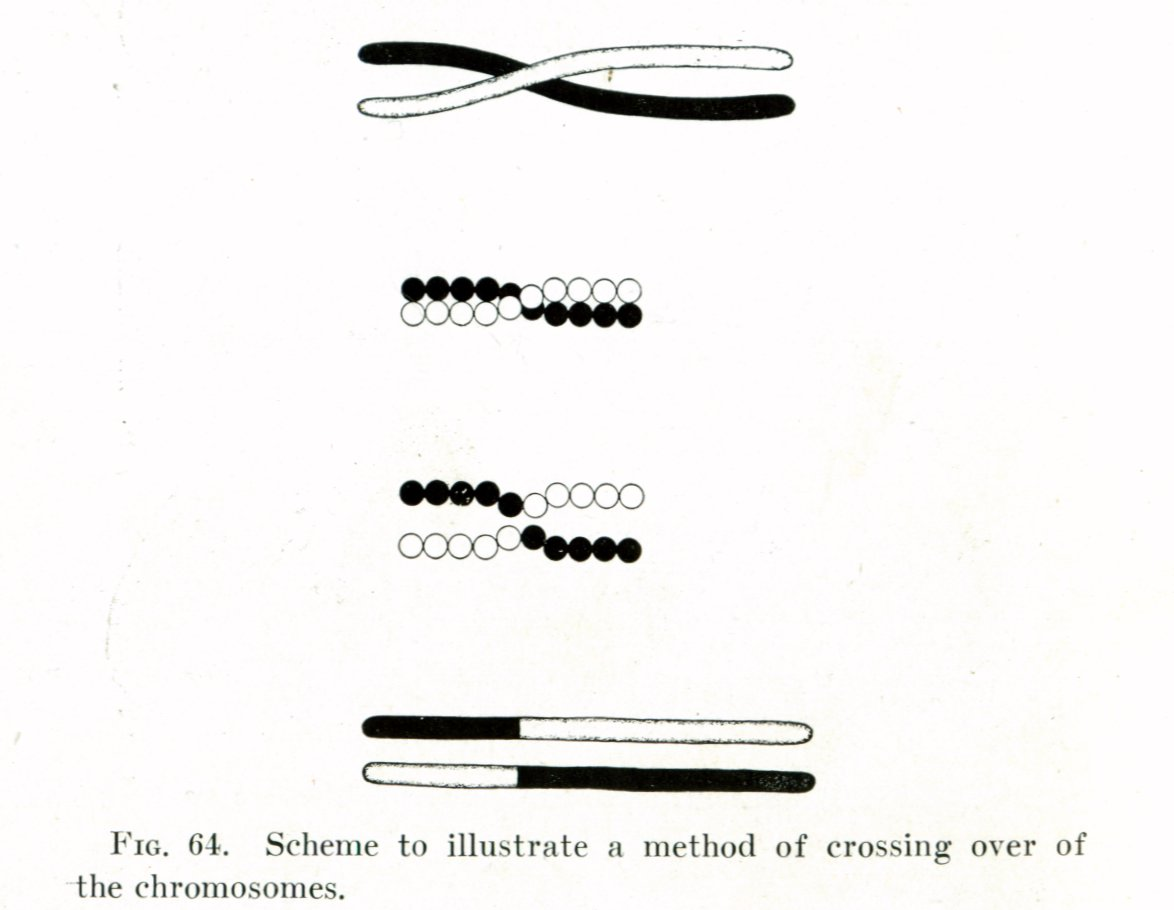
\includegraphics[height=1.2in]{res/crossover_morgan.jpg}
        \caption{Hình vẽ của T.H. Morgan về trao đổi chéo (1916)}
    \end{subfigure}
\end{figure}
\end{frame}

\begin{frame}{One-point crossover và N-point crossover}
  Ngoài one-point crossover, trao đổi chéo nhiều lần cũng xuất hiện trong tự
  nhiên, mặc dù hiếm gặp hơn. Mượn lấy ý tưởng này và tổng quát lên, ta có toán
  tử lai ghép \textbf{N-point crossover} (lai ghép $N$ điểm).

  Ý tưởng của toán tử này tương đối đơn giản: ta chọn lấy $N$ điểm cắt trên các
  nhiễm sắc thể cha mẹ, tạo ra $N + 1$ đoạn con trên mỗi nhiễm sắc thể, sau đó
  lấy xen kẽ các đoạn con để tạo ra các thể con.
\begin{figure}[t!]
    \centering
    \begin{subfigure}[t]{0.5\textwidth}
        \centering
        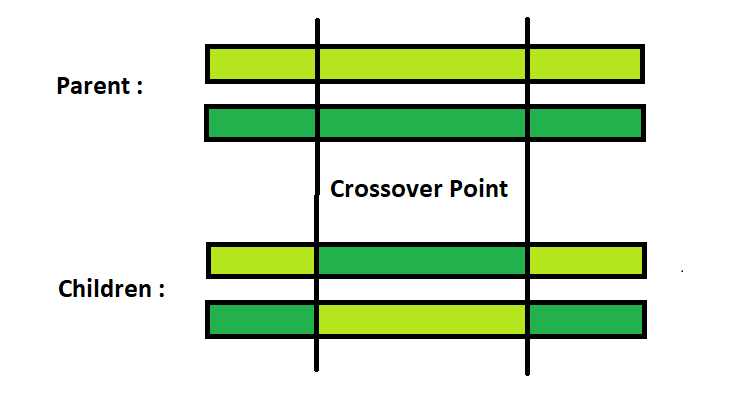
\includegraphics[height=1.2in]{res/2pco.png}
        \caption{Lai ghép hai điểm sinh ra hai cá thể con}
    \end{subfigure}%
    ~ 
    \begin{subfigure}[t]{0.5\textwidth}
        \centering
        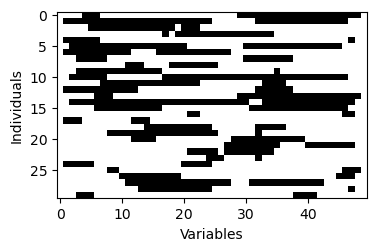
\includegraphics[height=1.2in]{res/4ptco.png}
        \caption{Các cá thể con sinh ra từ lai ghép 4 điểm}
    \end{subfigure}
\end{figure}
\end{frame}

\begin{frame}[fragile]
\frametitle{Uniform crossover}
  Một toán tử lai ghép đơn giản nữa là \textbf{Uniform crosover} (lai ghép đều).
  Mỗi gen của cá thể con sẽ được xác định bởi ngẫu nhiên, với xác suất 50\% là
  gen (cùng vị trí) của một cá thể cha mẹ và xác suất 50\% còn lại là gen cùng
  vị trí của cá thể cha mẹ còn lại.

  \begin{minted}{python}
import random

def ux(p1, p2):
  # tạo ra hai nhiễm sắc thể con là bản sao của cha mẹ
  c1 = list(p1)
  c2 = list(p2)
  for i in range(len(p1)):
    if random.random() < 0.5:
      swap(c1[i], c2[i])
  \end{minted}
\end{frame}

\begin{frame}[fragile]
\frametitle{Simulated Binary Crossover}
Vào năm 1995, Deb và Agrawal đã đề xuất ra toán tử Simulated Binary Crossover
(lai ghép nhị phân mô phỏng, SBX), mô phỏng lại toán tử One-point Crossover cho
các cá thể được mã hóa dưới dạng vector thực.

Toán tử này có các lợi thế hơn là thực hiện One-point Crossover trực tiếp trên
vector thực như giữ lại được những cấu trúc từ cá thể cha mẹ để chuyển sang đời
con, nên nó được ứng dụng rộng rãi trong giải các bài toán tối ưu phi tuyến.
\end{frame}

\begin{frame}[fragile]
\frametitle{Simulated Binary Crossover}
SBX hoạt động độc lập trên từng gen của hai nhiễm sắc thể cha mẹ. Do vậy, ta chỉ
cần xét SBX cho trường hợp số chiều bằng 1.

Giả sử hai cá thể cha mẹ (mã hóa là 2 số thực) \( p_{1}, p_{2} \) sinh ra hai cá
thể con là \( c_{1}, c_{2} \). Khi đó, theo cách làm của One-point crossover, ta
có được một bất biến:
\[
  p_{1} + p_{2} = c_{1} + c_{2}
.\] 
Như vậy, ta có thể đặc trưng một kết quả lai ghép bằng một tham số. Deb và
Agrawal sử dụng hệ số phủ (spread factor), được định nghĩa bởi:
\[
  \beta = \left| \frac{c_{1} - c_{2}}{p_{1} - p_{2}} \right| 
.\] 
\end{frame}

\begin{frame}[fragile]
\frametitle{Simulated Binary Crossover}
Từ hệ số phủ, ta dễ dàng tính lại các giá trị mã hóa của hai cá thể con:
\begin{align*}
  c_{1,2} &= \frac{1}{2}(p_{1} + p_{2}) \pm \frac{1}{2}\beta(p_{1} - p_{2})\\
  &= \frac{1}{2} \left[ (1 \pm \beta)p_{1} + (1 \mp \beta) p_{2}  \right]
.\end{align*}
Từ đây, ta có ý tưởng của SBX như sau: ta mô phỏng lai ghép nhị phân bằng cách lấy
ngẫu nhiên $\beta$ theo một phân phối nào đó, sau đó thay vào công thức để tính
ra giá trị mã hóa của các cá thể con.

Phân phối của \( \beta \) sẽ là một phân phối được lấy xấp xỉ với phân phối thực
của \( \beta \) suy ra từ thực nghiệm, và cách làm này cũng có thể được áp dụng
để mô phỏng các loại lai ghép khác.
\end{frame}

\begin{frame}[fragile]
\frametitle{Simulated Binary Crossover}
Deb và Agrawal xét giá trị \( \beta \) thu được bằng cách thực hiện One-point
Crossover với các nhiễm sắc thể mã hóa nhị phân, thu được hàm mật độ xác suất
(PDF) \( f_{\beta}(x) \) như sau:
\begin{figure}
  \centering
  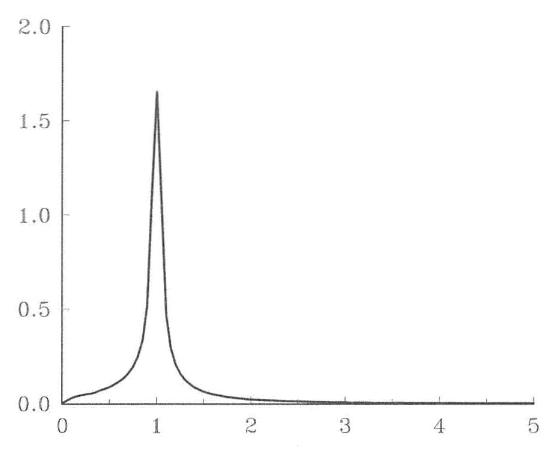
\includegraphics[height=.25\textheight]{res/sbx_pdf.png}
  \captionsetup{belowskip=0pt}
\end{figure}
Hai tác giả cho xác suất co và giãn bằng nhau, dẫn đến tính chất sau của hàm này:
\[
  f_{\beta} \left( \frac{1}{x} \right) = x^2 f_{\beta}(x), \forall x \in [0, 1]
,\] nghĩa là ta chỉ cần xác định giá trị của hàm này trên đoạn \( [0, 1] \).
\end{frame}

\begin{frame}[fragile]
\frametitle{Simulated Binary Crossover}
Do hình dạng của đồ thị hàm số \( f_{\beta} \) trên \( [0, 1] \), một lựa chọn
tự nhiên và linh hoạt để xấp xỉ hàm PDF là một hàm đa thức từng khoảng:
\[
  f_{\beta}(x) = \begin{cases}
    Cx^{\eta}, &\text{ nếu }x \in [0, 1]\\
    Cx^{-(\eta + 2)}, &\text{ nếu }x > 1
  \end{cases}
.\] 
Hệ số \( C \) dề dàng tính ra được là \( C = \frac{1}{2}(\eta  + 1) \). Số mũ \(
\eta 
\) được gọi là chỉ số của phân phối, \( \eta  \) lớn sẽ làm cho \( x \) được phân bố
dày đặc hơn ở xung quanh giá trị trung bình \( \bar{\beta} = 1 \).

Để tạo số ngẫu nhiên trong máy tính, ta sử dụng hàm ngược của hàm phân phối xác
suất (CDF), dễ dàng thu được từ hàm \( f_{\beta} \).
\[
  F^{-1}_{\beta}(\mu) = \begin{cases}
    (2\mu )^{1/(\eta  + 1)}, &\text{ nếu }\mu  < \frac{1}{2}\\
    (2(1 - \mu))^{-1/(\eta +1)}, &\text{ nếu ngược lại }
  \end{cases}
.\] 
\end{frame}

\begin{frame}[fragile]
\frametitle{Simulated Binary Crossover}
\begin{minted}[fontsize=\small]{python}
import random

eta = 3  # chỉ số phân phối
def sbx_single(p1, p2):
  mu = random.random()
  if mu < 0.5:
    beta = pow(2 * mu, 1 / (eta + 1)) 
  else:
    beta = pow(2 * (1 - mu), 1 / (eta + 1))
  return 0.5 * ((p1 + p2) + beta * (p1 - p2)),
         0.5 * ((p1 + p2) - beta * (p1 - p2))

def sbx(p1, p2):
  c1 = [0] * len(p1)
  c2 = [0] * len(p2)
  for i in range(len(p1)):
    c1[i], c2[i] = sbx_single(p1[i], p2[i])
  return c1, c2
\end{minted}
\end{frame}

\begin{frame}[fragile]
\frametitle{Order Crossover và Partially Mapped Crossover}
Các phép lai ghép trên sẽ sinh ra hai (hoặc một) cá thể con từ hai cá thể cha mẹ
với mã hóa nhiễm sắc thể dạng mảng. Tuy nhiên, nó không đảm bảo mảng nhiễm sắc
thể của cá thể con thỏa mãn những tính chất mà các cá thể cha mẹ đã có.

Với bài toán đường đi Hamilton, nhiễm sắc thể hợp lệ cần phải có các phần tử
khác nhau, hoặc nói cách khác là một hoán vị của tập số chỉ của các đỉnh đồ thị.
Do đó, để giải quyết các bài toán này, ta cần có một phép lai ghép bảo toàn tính
chất của hoán vị từ đời cha mẹ sang đời con.

Hai toán tử \textbf{Order Crossover} (OX1) và \textbf{Partially Mapped
Crossover} (PMX) là hai toán tử lai ghép cho các hoán vị, bảo đảm không sinh ra
các phần tử trùng lặp.
\end{frame}

\begin{frame}[fragile]
\frametitle{Order Crossover và Partially Mapped Crossover}
\begin{itemize}
\item 
OX1 đầu tiên chọn ra một số gen (hoặc đoạn gen) trên cá thể cha mẹ đầu tiên (\(
p_{1}\)) sẽ
được chuyển thẳng sang cá thể con. Các vị trí gen còn lại trên cá thể con được
xác định thông qua việc điền các gen còn thiếu theo thứ tự xuất hiện trên cá thể
cha mẹ còn lại \( p_{2} \).

\item
PMX chọn ra một đoạn gen trên cá thể cha mẹ đầu tiên \( p_{1} \) để chuyển thẳng
sang cá thể con. Các gen nằm trên vị trí tương ứng của cá thể cha mẹ còn lại (\(
p_{2}\)), mà không xuất hiện trên đoạn được chuyển sẽ được hoán đổi vị trí với
các gen được chuyển có vị trí trên \( p_{2} \) nằm ngoài đoạn này. Các gen còn
lại có thể được chuyển thẳng từ \( p_{2} \) mà vẫn đảm bảo tính chất của hoán
vị.
\end{itemize}
\end{frame}


\begin{frame}[fragile]
\frametitle{Order Crossover và Partially Mapped Crossover}
\begin{itemize}
\item 
OX1 đầu tiên chọn ra một số gen (hoặc đoạn gen) trên cá thể cha mẹ đầu tiên (\(
p_{1}\)) sẽ
được chuyển thẳng sang cá thể con. Các vị trí gen còn lại trên cá thể con được
xác định thông qua việc điền các gen còn thiếu theo thứ tự xuất hiện trên cá thể
cha mẹ còn lại \( p_{2} \).
\begin{align*}
  p_{1} &= (1, 2, \underline{3, 4}, 5) \\
  p_{2} &= (3, 5, 2, 4, 1)\\
  \implies c &= (?, ?, \underline{3, 4}, ?) \\
  p_{2}' &= (\cancel{3}, 5, 2, \cancel{4}, 1) \to  (5, 2, 1) \\
  \implies c&= (\underline{5, 2}, 3, 4, \underline{1})
.\end{align*}

Lượng thông tin di truyền chuyển giao từ cá thể cha mẹ sang cá thể con có thể
được cải thiện bằng cách cải tiến toán tử này thành toán tử \textbf{Order-based
Crossover} (OX2) hoặc \textbf{Position-based Crossover} (POS).
\end{itemize}
\end{frame}

\begin{frame}[fragile]
\frametitle{Order Crossover và Partially Mapped Crossover}
\begin{itemize}
\item 
PMX chọn ra một đoạn gen trên cá thể cha mẹ đầu tiên \( p_{1} \) để chuyển thẳng
sang cá thể con. Các gen nằm trên vị trí tương ứng của cá thể cha mẹ còn lại (\(
p_{2}\)), mà không xuất hiện trên đoạn được chuyển sẽ được hoán đổi vị trí với
các gen được chuyển có vị trí trên \( p_{2} \) nằm ngoài đoạn này. Các gen còn
lại có thể được chuyển thẳng từ \( p_{2} \) mà vẫn đảm bảo tính chất của hoán
vị.
\begin{align*}
  p_{1} &= (1, 2, 3, \underline{4, 5, 6}, 7, 8) \\
  p_{2} &=  (3, 7, 5, 1, 6, 8, 2, 4) \\
  \implies c &= (?, ?, ?, \underline{4, 5, 6}, ?, ?) \\
  p_{2}' &= (\cdot, \cdot, \cdot, \underline{\mathbf{1}, 6, \mathbf{8}}, \cdot,
  \cdot) \\
  p_{2}'' &= (\cdot, \cdot, 5, \cdot, \cdot, \cdot, \cdot, 4) \\
  \implies c &= (?, ?, 8, 4, 5, 6, ?, 1) \\
  \implies c&= (3, 7, 8, 4, 5, 6, 2, 1)
.\end{align*}
\end{itemize}
\end{frame}

% subsection Toán tử lai ghép (end)

\subsection{Toán tử đột biến} % (fold)
\label{sub:Toán tử đột biến}

\begin{frame}{Toán tử đột biến}
Toán tử đột biến nhằm tăng tính đa dạng cho quần thể bằng cách ngẫu nhiên làm
gây ra những thay đổi nhỏ trong cấu trúc gen của các nhiễm sắc thể.

Trong sinh học, có đột biến cấu trúc nhiễm sắc thể, nhưng do ta đang xét một cá
thể là một nhiễm sắc thể, nên cách làm này không phù hợp. Trong đột biến gen còn
có các dạng đột biến như thêm, bớt, làm thay đổi độ dài của nhiễm sắc thể, nên
cũng ít được sử dụng trong các giải thuật tiến hóa.

Vì vậy, toán tử đột biến trong các giải thuật tiến hóa thường được mô hình theo
dạng đột biến thay thế một hoặc một số gen.

\end{frame}
\begin{frame}{Toán tử đột biến}
\begin{figure}
  \centering
  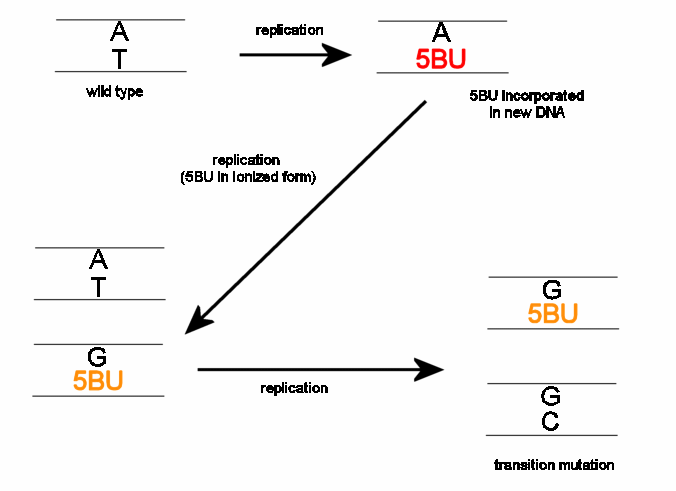
\includegraphics[width=.8\textwidth,height=0.7\textheight,keepaspectratio]
  {res/5bu.png}
  \caption{Đột biến thay thế gen xảy ra do 5BU (5-Bromouracil)}
\end{figure}
\end{frame}

\begin{frame}[fragile]
\frametitle{Bit String Mutation}
  \textbf{Bit String Mutation} là toán tử đột biến đơn giản nhất. Nó mô phỏng
  lại quá trình đột biến thay thế gen bằng cách đảo một (hoặc một số) gen
  được chọn ngâu nhiên trên nhiễm sắc thể.
  \begin{align*}
    b &= (0, 1, 0, \mathbf{0}, 1, 0) \in \{0, 1\} ^{6}\\
    \to b' &= (0, 1, 0, \mathbf{1}, 1, 0)
  .\end{align*}

  \begin{minted}{python}
import random

def bit_string_mutate(x):
  for i in range(len(x)):
    if random.random() < bit_string_mutate_rate:
      # đảo bit ngẫu nhiên
      x[i] = not(x[i])
  \end{minted}
\end{frame}

\begin{frame}[fragile]
\frametitle{Đột biến vector thực nhờ phân phối chuẩn}
Khi mở rộng Bit String Mutation cho các loại mã hóa phức tạp hơn như vector số
thực, ta sẽ gặp phải vấn đề là không biết chọn giá trị nào để thay thế cho những
gen được chọn ngẫu nhiên.

Một cách tự nhiên để giải quyết vấn đề này là tạo ra một gen ngẫu nhiên thay thế
cho mỗi gen đột biến.

Một cách thông dụng hơn là sử dụng một biến ngẫu nhiên phân phối chuẩn để cộng
thêm vào gen đột biến:
\[
  x \coloneqq  x + \Delta x,\, \Delta x \sim \mathcal{N}(0, \sigma)
.\] 

Biến ngẫu nhiên này tượng trung cho lượng nhiễu (noise) sinh ra do đột biến,
được mô phỏng qua phân phối chuẩn.
\end{frame}

\begin{frame}[fragile]
\frametitle{Đột biến vector thực nhờ phân phối chuẩn}
Nếu gen \( x \) cần nằm trong đoạn \( [a, b] \), thì độ lệch chuẩn của biến ngẫu
nhiên \( \Delta x \) có thể được tính thông qua độ dài của đoạn này:
\[
  \sigma = \frac{b - a}{6}
.\] 

Mẫu số \( 6 \) nảy sinh trong tính toán. Theo luật \( 68-95-99.7 \) trong thống
kê, thì khoảng \( 99.7\% \approx 100\% \) các giá trị trong phân phối chuẩn
cách xa giá trị trung bình nhiều nhất \( 3\sigma \). Do đó, \( [- 3\sigma, 
3\sigma] \), chứa hầu như tất cả các giá trị đáng kể của phân phối này, nên một
cách tự nhiên, ta sẽ muốn khoảng này có cùng độ dài với khoảng giá trị của \( x
\).

Sau khi cộng \( \Delta x \) vào gen \( x \), ta cần phải "kẹp" (clamp) lại biến
\( x \) này trong khoảng giá trị của nó, không cho phép nó ra ngoài \( [a, b]
\).
\end{frame}

\begin{frame}[fragile]
\frametitle{Relative Parameter Mutation}
Vì tạo số ngẫu nhiên theo phân phối chuẩn tương đối kém hiệu quả trên máy tính,
người ta đề xuất ra một cách đột biến tương tự, gọi là \textbf{Relative
Parameter Mutation} (đột biến tham số tương đối).
\begin{itemize}
\item Đầu tiên, ta xác định nên tăng hay giảm giá trị của gen này bằng một biến
  ngẫu nhiên với xác suất bằng nhau.
\item Giả sử như ta tiến hành tăng giá trị cho gen, nghĩa là giá trị mới \( x'
  \) phải nằm trong đoạn \( [x, b] \).
\item Ta xét \( k \) đoạn \( I_{i} = \left[ x, \frac{i}{k}(b - x) \right], i \in
  \{1, 2, \ldots ,k\}  \), và chọn ra một đoạn ngẫu nhiên trong những đoạn này.
  Sau đó, ta tiếp tục chọn ra một số ngẫu nhiên từ đoạn vừa chọn và lấy đây làm
  giá trị mới cho gen.
\end{itemize}

  Cách làm này, giống như cách sử dụng phân phối chuẩn cũng làm xuất hiện
  nhiều thay đổi nhỏ hơn là thay đổi lớn, do giá trị mới gần với giá trị cũ sẽ
  nằm ở trong nhiều đoạn \( I_{i} \) hơn và sẽ có xác suất được chọn cao hơn.
\end{frame}

\begin{frame}[fragile]
\frametitle{Polynomial Mutation}
Một hướng khác cải thiện cho cách đột biến dùng phân phối chuẩn là sử dụng một
phân phối khác dễ tính hơn. Chẳng hạn, \textbf{Polynomial Mutation} dựa vào phân
phối của biến \( \beta \) trong SBX để tính \( \Delta x \):
\begin{align*}
  \Delta x = \beta' \Delta x_{\text{max}}
.\end{align*}

Ở đây, \( \beta' \) nằm trong đoạn \( [-1, 1] \), khác với \( \beta \in [0,
+\infty) \), nên ta cần có điều chỉnh lại công thức tính \( \beta \) thành:
\[
  F^{-1}_{\beta'}(\mu) = \begin{cases}
    (2x)^{1 / (n+1)} - 1, &\text{ nếu }\mu < \frac{1}{2}\\
    -(2(1 - x))^{1 / (n+1)} + 1, &\text{ nếu ngược lại }
    
  \end{cases}
.\] 
\end{frame}

\begin{frame}[fragile]
\frametitle{Đột biến cho hoán vị}
Các toán tử đột biến không bảo toàn tính chất của hoán vị, nên với cách mã hóa
các nhiễm sắc thể bằng một hoán vị, cần sử dụng các toán tử đột biến đặc biệt:
\begin{itemize}
\item Đột biến Twors: đổi chỗ hai gen bất kì trên nhiễm sắc thể.
  \[
  x = (\underline{1}, 2, \underline{3}, 4) \to x' = (\underline{3}, 2,
  \underline{1}, 4)
  .\] 
\item Đột biến trượt: chọn một dãy gen con của nhiễm sắc thể, sau đó trượt
  (rotate) các gen trong dãy này.
  \[
    x = (\underline{1, 2, 3}, 4) \to x' = (\underline{3, 1, 2}, 4)
  .\] 
\item Đột biến đảo: chọn một dãy gen con của nhiễm sắc thể, sau đó đảo ngược thứ
  tự các gen trong dãy này.
  \[
    x = (\underline{1, 2, 3}, 4) \to x' = (\underline{3, 2, 1}, 4)
  .\] 
\end{itemize}
\end{frame}
% subsection Toán tử đột biến (end)

\subsection{Ứng dụng giải thuật di truyền để giải bài toán người bán hàng} % (fold)
\label{sub:Ứng dụng giải thuật di truyền để giải bài toán người bán hàng}

\begin{frame}{Ứng dụng giải thuật di truyền để giải bài toán người du lịch}
  Việc sử dụng giải thuật di truyền cho một bài toán chỉ gồm \textbf{chọn các
  toán tử di truyền phù hợp}, \textbf{khởi tạo quần thể}  và \textbf{cài đặt hàm
  fitness}.

  Trong phần này, ta xét một ví dụ cụ thể: bài toán người bán hàng (Travelling
  Salesman Problem, TSP). Cho một đồ thị \( G = (V, E) \), mỗi cạnh \( e \in E \) có
  tương ứng một độ dài \( \ell(e) \). Bài toán TSP cần tìm ra chu trình
  Hamilton (đi qua mọi đỉnh của đồ thị đúng một lần) có độ dài các cạnh là nhỏ
  nhất:
  \[
\begin{aligned}
  &&\min\, \ell(C) &= \sum_{i = 1}^{n} \ell(v_{i}v_{i+1})\\
  &&\text{subject to}\, C &= v_{1}v_{2}\ldots v_{n}v_{1},\\
  &&{} V &= \{v_{1}, v_{2}, \ldots , v_{n}\}, \\
  &&{} v_{n+1} &= v_{1}; v_{i}v_{i + 1} \in E, \forall i=\overline{1,n}\\
  && (n &= |V|)
.\end{aligned}
  \] 
\end{frame}

\begin{frame}[fragile]
\frametitle{Ứng dụng giải thuật di truyền để giải bài toán người du lịch}
  Cài đặt hàm fitness chỉ đơn thuần là tính tổng độ dài các cạnh theo công thức:
  \begin{minted}{python}
def fitness(cycle):
  return sum(length(cycle[i], cycle[i + 1])
             for i in range(-1, len(cycle) - 1))
  \end{minted}

  Khởi tạo các cá thể ngẫu nhiên cũng chỉ đơn thuần là tạo ra một hoán vị ngẫu
  nhiên của tập đỉnh. Vậy ta chỉ còn lại việc tìm các toán tử thích hợp:

  \begin{itemize}
  \item Chọn lọc: mọi cách chọn lọc đều có thể sử dụng được.
  \item Lai ghép: các cách lai ghép cho hoán vị đều có thể sử dụng được. Ta có
    thể chọn OX1 hoặc PMX.
  \item Đột biến: để đơn giản, ta có thể sử dụng đột biến Twors.
  \end{itemize}
\end{frame}
% subsection Ứng dụng giải thuật di truyền để giải bài toán người du lịch (end)

